\section{Методы регистрации экзопланет, преимущества и недостатки разных методов.}
\subsection{Изменение лучевой скорости звезды (вращение вокруг центра масс системы звезда-планета)
}
Смотрим на спектр звезды вокруг которой вращается экзопланета, за счет эффекта Доплера спектр будет вмещаться в синюю/красную сторону, когда движется к нам/от нас 
Благодаря этому измеряем орбитальный период звезды, орбитальный период планеты, соответсвенно, такой же. Зная массу звезды находим массу экзопланеты

Ситуация осложняется, когда планет много. 
\subsection{Транзитный метод}
Визуально, конечно, не можем увидеть. Наблюдаются флуктуации блеска звезды. Блеск падает на очень маленькую величину (1000-ые доли), также мешает земная атмосфера, тем не менее изменения все равно регистрируются, особенно для крупных экзопланет, сейчас транзиты наблюдают со спутников.

Вероятность транзита составляет порядка 1\% (ДЗ 3).

\paragraph{Задача}
Рассчитайте вероятность транзита, если радиус звезды равен $R_{\star} = 0.5 R_{\Sun}$ ($R_{\Sun}$ -- радиус Солнца),
а большая полуось (круговой) орбиты $a = 0.1$ а.е. Радиус планеты $R_{\circ} = 1.4R_{\Jupiter}$ ($R_{\Jupiter}$ -- радиус
Юпитера). 
Положение наблюдателя считать случайным с равновероятным распределением. Отдельно рассчитать вероятность полного транзита $\mathcal{P}_{whole}$ (весь диск планеты проецируется на диск звезды) и частичного $\mathcal{P}_{partial}$, а также суммарную вероятность $\mathcal{P}_{\Sigma}$.
\paragraph*{Решение:}
\begin{figure}[H]
    \centering
    \begin{tikzpicture}[scale=1.5,>=latex']
    \filldraw[blue!22!white] (4.8,2*0.1032795559) -- (4,0) -- (4.8,-2*0.1032795559) -- cycle;
    \filldraw[blue!22!white] (-1,1.290994449) -- (4,0) -- (-1,-1.290994449) -- cycle;
    \filldraw[fill=yellow!55!white] (0,0) circle (1);
    \filldraw[] (0,0) circle (0.02);
    \draw[<->] (-1,0) -- (0,0) node[above,pos=0.5]{$R_{\star}$};
    \filldraw[xshift=4.4cm,fill=black!55!white] (0,0) circle (0.1); 
    \draw[xshift=4.4cm] (-0.1,0.2) -- (-0.1,-1);
    \draw[xshift=4.4cm] (0.1,0.2) -- (0.1,-1);
    \draw[xshift=4.4cm,->] (-0.5,-0.9) -- (-0.1,-0.9);
    \draw[xshift=4.4cm,->] (0.5,-0.9) -- (0.1,-0.9);
    \node[] at (4.4,-1.2){$2R_{\circ}$};
    %\draw (0.25,0.9682458) -- (0,0);
    \draw[] (-1,1.290994449) -- (4.8,-2*0.1032795559);
    \draw[] (-1,-1.290994449) -- (4.8,2*0.1032795559);
    \draw[dashed] (-1,1.23056316956) -- (48.4/9,-0.0978857);
    \draw[dashed] (-1,-1.23056316956) -- (48.4/9,0.0978857);
    \draw (0,0) -- (0,1.5);
    \draw[xshift=4.4cm] (0,0) -- (0,1.5);
    \draw[<-] (0,1.3) -- (2.1,1.3);
    \draw[->] (2.3,1.3) -- (4.4,1.3);
    \node at (2.2,1.3) {$a$};
    %\draw[<-] (0,0) -- (2.1,0);
    %\draw[->] (2.3,0) -- (4.4,0);
    %\node at (2.2,0) {$a$};
    \filldraw[xshift=4.4cm] (0,0) circle (0.02);
    \end{tikzpicture}
    \caption{Рисунок к задаче 1. Планета (тёмно-серая) может проецироваться на звезду (жёлтая) полностью (голубая область), а может частично (выделена пунктиром).}
    \label{prmlm_1pic}
\end{figure}
Из рисунка~\ref{prmlm_1pic} легко получить соотношения для вероятностей и их значения, учитывая $R_{\Sun} \approx 10R_{\Jupiter} =\approx 0.47\cdot10^{-2} $ а.е.:
\begin{multline*}
    \mathcal{P}_{whole} = \frac{R_{\star} - R_{\circ}}{a} = \frac{0.5R_{\Sun} - 1.4R_\Jupiter}{a} \approx \frac{0.5R_{\Sun} - 0.14_{\Sun}}{a} =\\ = \frac{0.36R_{\Sun}}{a} \approx \frac{0.36\cdot 0.47\cdot 10^{-2}}{0.1} \approx \boxed{1.7\%} 
\end{multline*}
\begin{multline*}
    \mathcal{P}_{\Sigma} = \frac{R_{\star} + R_{\circ}}{a} = \frac{0.5R_{\Sun} + 1.4R_\Jupiter}{a} \approx \frac{0.5R_{\Sun} + 0.14_{\Sun}}{a} =\\ = \frac{0.64R_{\Sun}}{a} \approx \frac{0.64\cdot 0.47\cdot 10^{-2}}{0.1} \approx \boxed{3.0\%} 
\end{multline*}
\begin{equation*}
    \mathcal{P}_{partial} = \mathcal{P}_{\Sigma} - \mathcal{P}_{whole} = 3.0 - 1.7 = \boxed{1.3\%}
\end{equation*}
\subsection{Микролинзирование}
Если близко к лучу зрения между наблюдаемой звездой и наблюдателем попадает объект (может быть что угодно, планетах черная дыра и тд), то объект искажает пространство-время вокруг себя, работает как гравитационная линза. Блеск звезды будет возрастать по мере того как линза будет все ближе подлетать к лучу зрения, а потом симметрично убывать.

 Если линза состоит из нескольких объектов, в нашем случае массивная звезда и экзопланета, то в изменении регистрируемого блеска будет возникать небольшой пик от планеты.

Плюс метода в том что единичное наблюдение гарантирует результат, не нужно долго копить данные. Линзирования также работает на очень удалённых объектах, что нехарактерно в других методах. 
\begin{figure}[H]
    \centering
    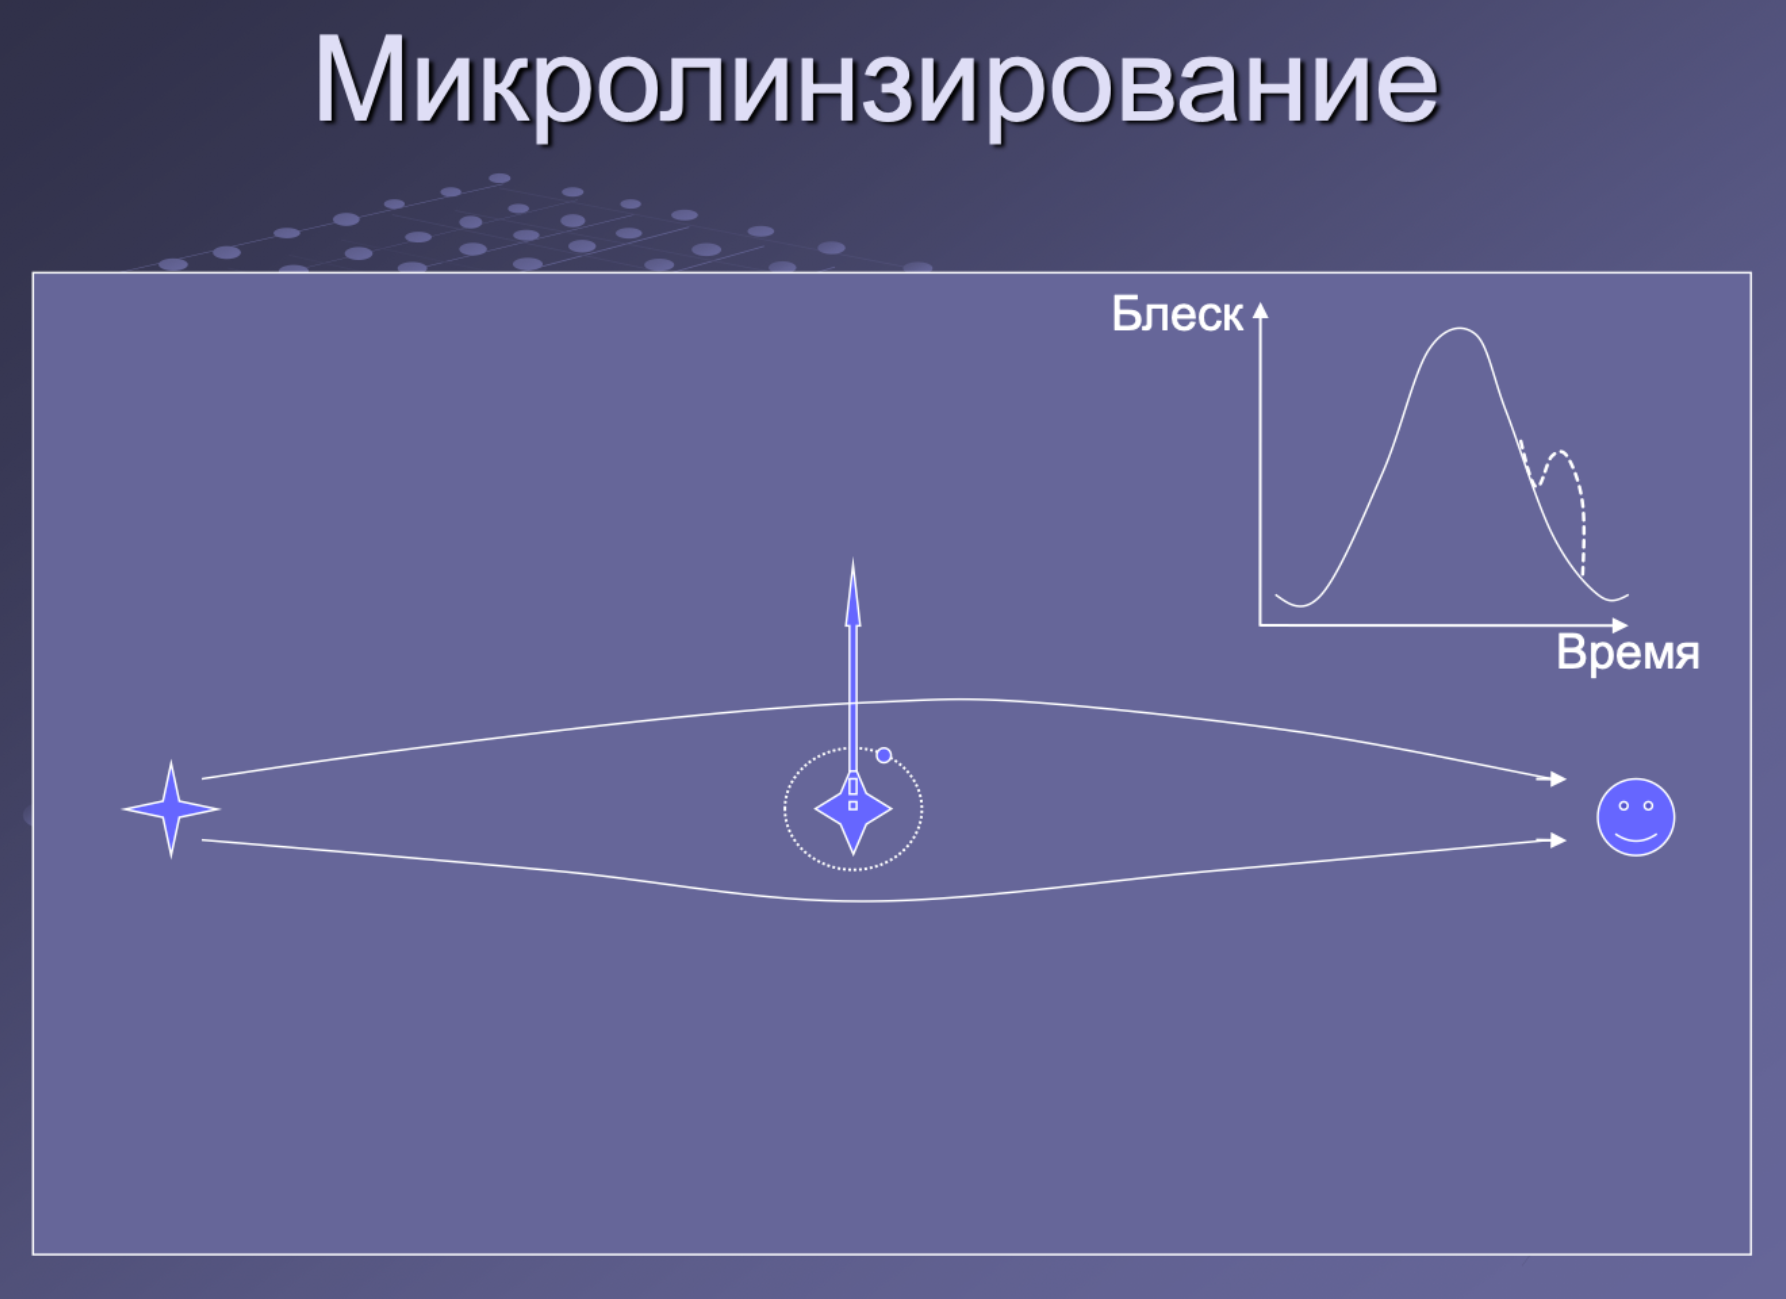
\includegraphics[scale=0.4]{5_mcrl.png}
    \caption{Микролинзирование}
    \label{fig:mcrl}
\end{figure}
\subsection{Тайминг}
Если мы наблюдаем систему в которой происходят какие-то периодические события, то наличие внешних объектов буду приводить к изменению преиода. Например, для пульсаров будет возникать эффект доплера из-за вращения вокруг центра масс системы пульсар-экзопланета.

\subsection{Астрометрическое детектирование}
Самый старый и неточный способ. Мы не видим планету, но можем измерить, что меняется положение звезды, т.к. она вращается вокруг центра масс системы. Метод требует очень высокой точности измерений 
\subsection{Выделение вклада планеты в общее излучение системы}
Например, в случае транзитной планеты (если она является достаточно мощным
 источником собственного или отраженного излучения) мы можем увидеть не только падение блеска системы при транзите, но и рост блеска в те моменты, когда одновременно виден и весь диск звезды, и диск планеты. Таким способом удалось изучить свойства нескольких планет, например в системе Кеплер-70. Вклад планеты можно выделить и изучая спектры. Линии, излучаемые планетой, во-первых, будут соответствовать другим скоростям и смещаться (из-за эффекта Доплера) относительно звездных линий. А во- вторых, по свойствам линий можно понять, что они связаны с относительно холодным веществом. Этот метод также успешно используется. В нескольких десятках случаев удалось получить непосредственные изображения молодых экзопланет.
\subsection{Непосредственное наблюдение}
Эти методом можно обнаружить только очень крупные, нагретые, удалённые от звезды планеты в силу того, что планеты являются очень слабыми источниками. Не смотря на ограниченные возможности этого метода таким способом обнаружено несколько десятков планет.
